\clearpage
\begin{textbox}{\href{https://compneuro.neuromatch.io/tutorials/W1D4_GeneralizedLinearModels/student/W1D4_Tutorial1.html}{The Leaky Integrate-and-Fire (LIF) Neuron Model } }
\begin{subbox}{subbox}{The Leaky Integrate-and-Fire (LIF) model}
\scriptsize
The basic idea of LIF neuron was proposed in 1907 by Louis Édouard Lapicque, long before we understood the electrophysiology of a neuron (see a translation of \href{https://pubmed.ncbi.nlm.nih.gov/17968583/}{Lapicque's paper}. 

The subthreshold membrane potential dynamics of a LIF neuron is described by

\begin{eqnarray}
C_m\frac{dV}{dt} = -g_L(V-E_L) + I
\end{eqnarray}

where $C_m$ is the membrane capacitance, $V$ is the membrane potential, $g_L$ is the leak conductance ($g_L = 1/R$, the inverse of the leak resistance $R$ mentioned in previous tutorials), $E_L$ is the resting potential, and $I$ is the external input current. 

Dividing both sides of the above equation by $g_L$ gives

\begin{align}
\tau_m\frac{dV}{dt} = -(V-E_L) + \frac{I}{g_L}\,,\quad (\ddagger)
\end{align}

where the $\tau_m$ is membrane time constant and is defined as $\tau_m=C_m/g_L$. 

Note that dividing capacitance by conductance gives units of time! 

Below, we will use Eqn.($\ddagger$) to simulate LIF neuron dynamics. 

If $I$ is sufficiently strong such that $V$ reaches a certain threshold value $V_{\rm th}$, $V$ is reset to a reset potential $V_{\rm reset}< V_{\rm th}$, and voltage is clamped to $V_{\rm reset}$ for $\tau_{\rm ref}$ ms, mimicking the refractoriness of the neuron during an action potential:

\begin{eqnarray*}
\mathrm{if}\quad V(t_{\text{sp}})\geq V_{\rm th}&:& V(t)=V_{\rm reset} \text{  for } t\in(t_{\text{sp}}, t_{\text{sp}} + \tau_{\text{ref}}]
\end{eqnarray*}
where $t_{\rm sp}$ is the spike time when $V(t)$ just exceeded $V_{\rm th}$.

\centering
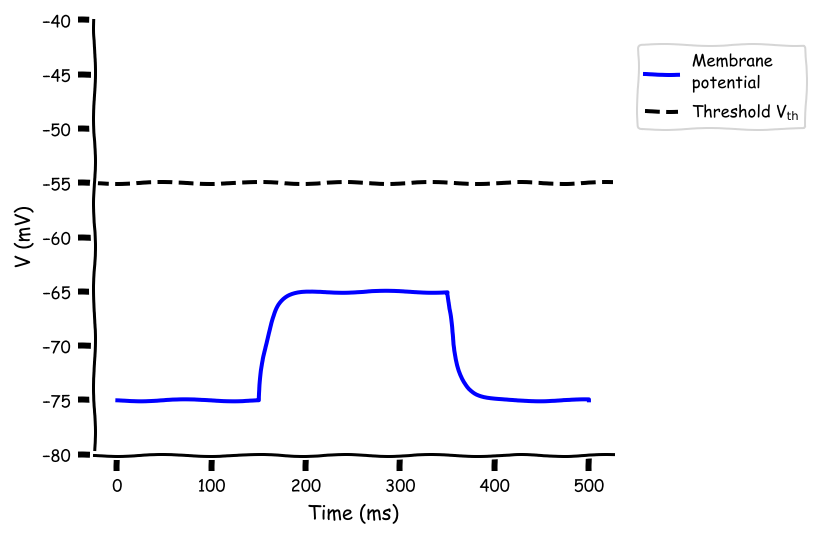
\includegraphics[scale=0.15]{Figures/BNM/LIF_Figure1.png}
\end{subbox}

\end{textbox}
%%%%%%%%%%%%%%%%%%%%%%%%%%%%%%%%%%%%%%%%%%%%%%%%%%
%%%%%%%%%%%%%%%%%%%%%%%%%%%%%%%%%%%%%%%%%%%%%%%%%%
\begin{textbox}{\href{https://compneuro.neuromatch.io/tutorials/W1D4_GeneralizedLinearModels/student/W1D4_Tutorial1.html}{The Leaky Integrate-and-Fire (LIF) Neuron Model } }
\begin{subbox}{subbox}{Response of an LIF model to different types of input currents}
\scriptsize
In the following section, we see how to inject direct current and white noise to study the response of an LIF neuron.
The neuron generates a spike. But this is just a cosmetic spike only for illustration purposes. In an LIF neuron, we only need to keep track of times when the neuron hits the threshold so the postsynaptic neurons can be informed of the spike. 

\centering
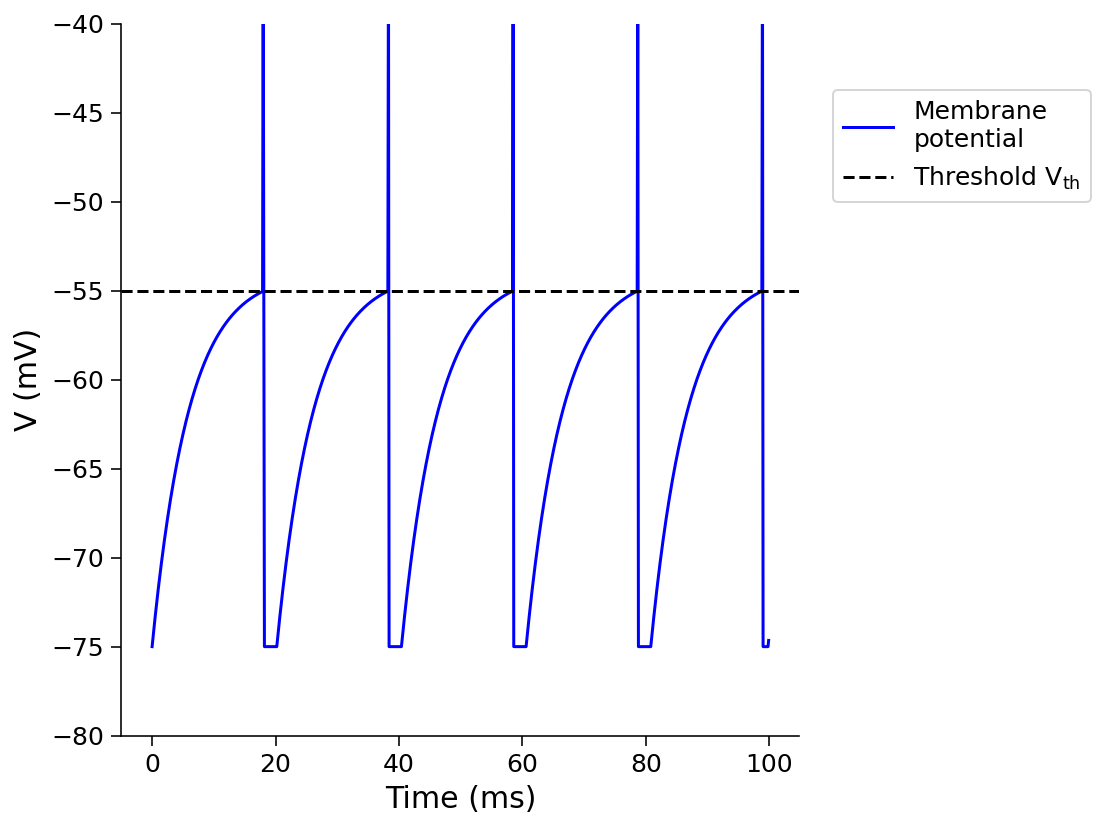
\includegraphics[scale=0.2]{Figures/BNM/LIF_Figure2.png}
\end{subbox}

\begin{subbox}{subbox}{Gaussian white noise (GWN) current 
}
\scriptsize
Given the noisy nature of neuronal activity \textit{in vivo}, neurons usually receive complex, time-varying inputs.

To mimic this, we will now investigate the neuronal response when the LIF neuron receives Gaussian white noise $\xi(t)$ with mean 0 ($\mu = 0$) and some standard deviation $\sigma$.

Note that the GWN has zero mean, that is, it describes only the fluctuations of the input received by a neuron. We can thus modify our definition of GWN to have a nonzero mean value $\mu$ that equals the DC input, since this is the average input into the cell. The cell below defines the modified gaussian white noise currents with nonzero mean $\mu$.

\centering
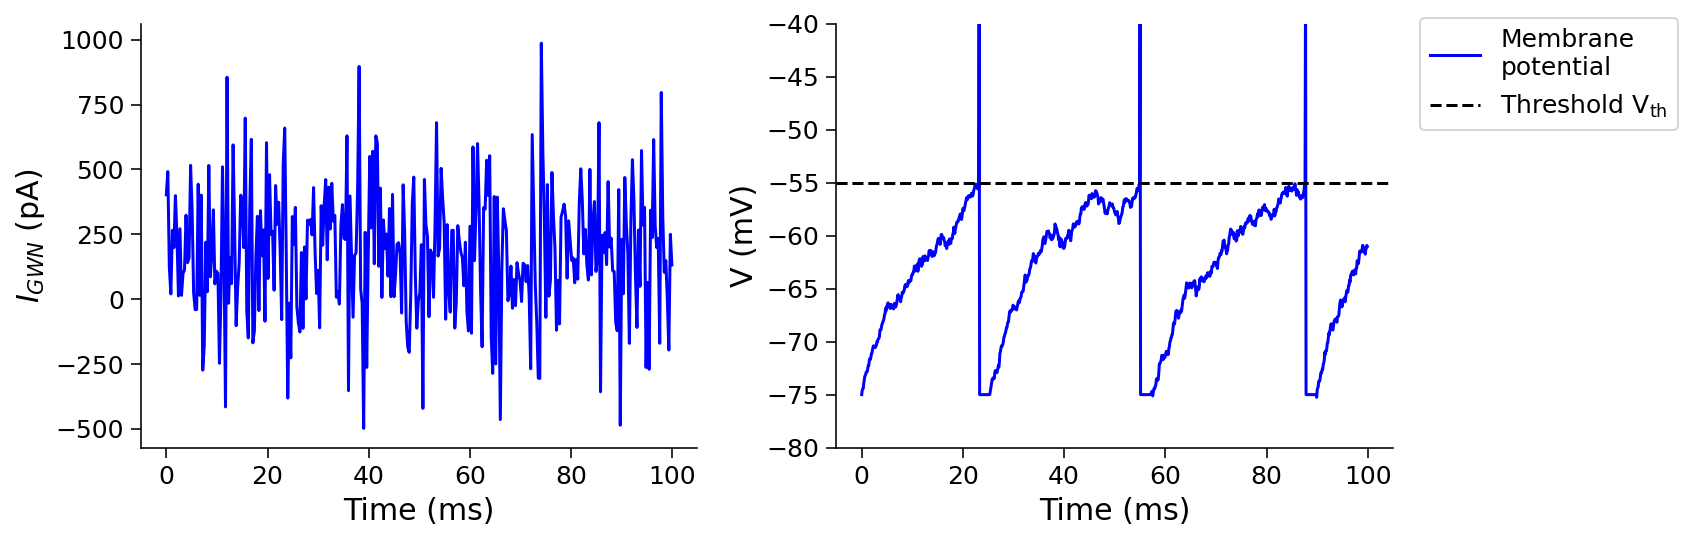
\includegraphics[scale=0.25]{Figures/BNM/LIF_Figure3.png}
\end{subbox}
\end{textbox}

%%%%%%%%%%%%%%%%%%%%%%%%%%%%%%%%%%%%%%%%%%%%%%%%%%
%%%%%%%%%%%%%%%%%%%%%%%%%%%%%%%%%%%%%%%%%%%%%%%%%%
\begin{textbox}{\href{https://compneuro.neuromatch.io/tutorials/W1D4_GeneralizedLinearModels/student/W1D4_Tutorial1.html}{The Leaky Integrate-and-Fire (LIF) Neuron Model } }
\begin{subbox}{subbox}{Firing rate and spike time irregularity}
\scriptsize
When we plot the output firing rate as a function of GWN mean or DC value, it is called the input-output transfer function of the neuron (so simply F-I curve).

Spike regularity can be quantified as the \textbf{coefficient of variation (CV) of the interspike interval (ISI)}:
\begin{align}
\text{CV}_{\text{ISI}} = \frac{std(\text{ISI})}{mean(\text{ISI})}
\end{align}

A Poisson train is an example of high irregularity, in which $\textbf{CV}_{\textbf{ISI}} \textbf{= 1}$. And for a clocklike (regular) process we have $\textbf{CV}_{\textbf{ISI}} \textbf{= 0}$ because of \textbf{std(ISI)=0}.

\centering
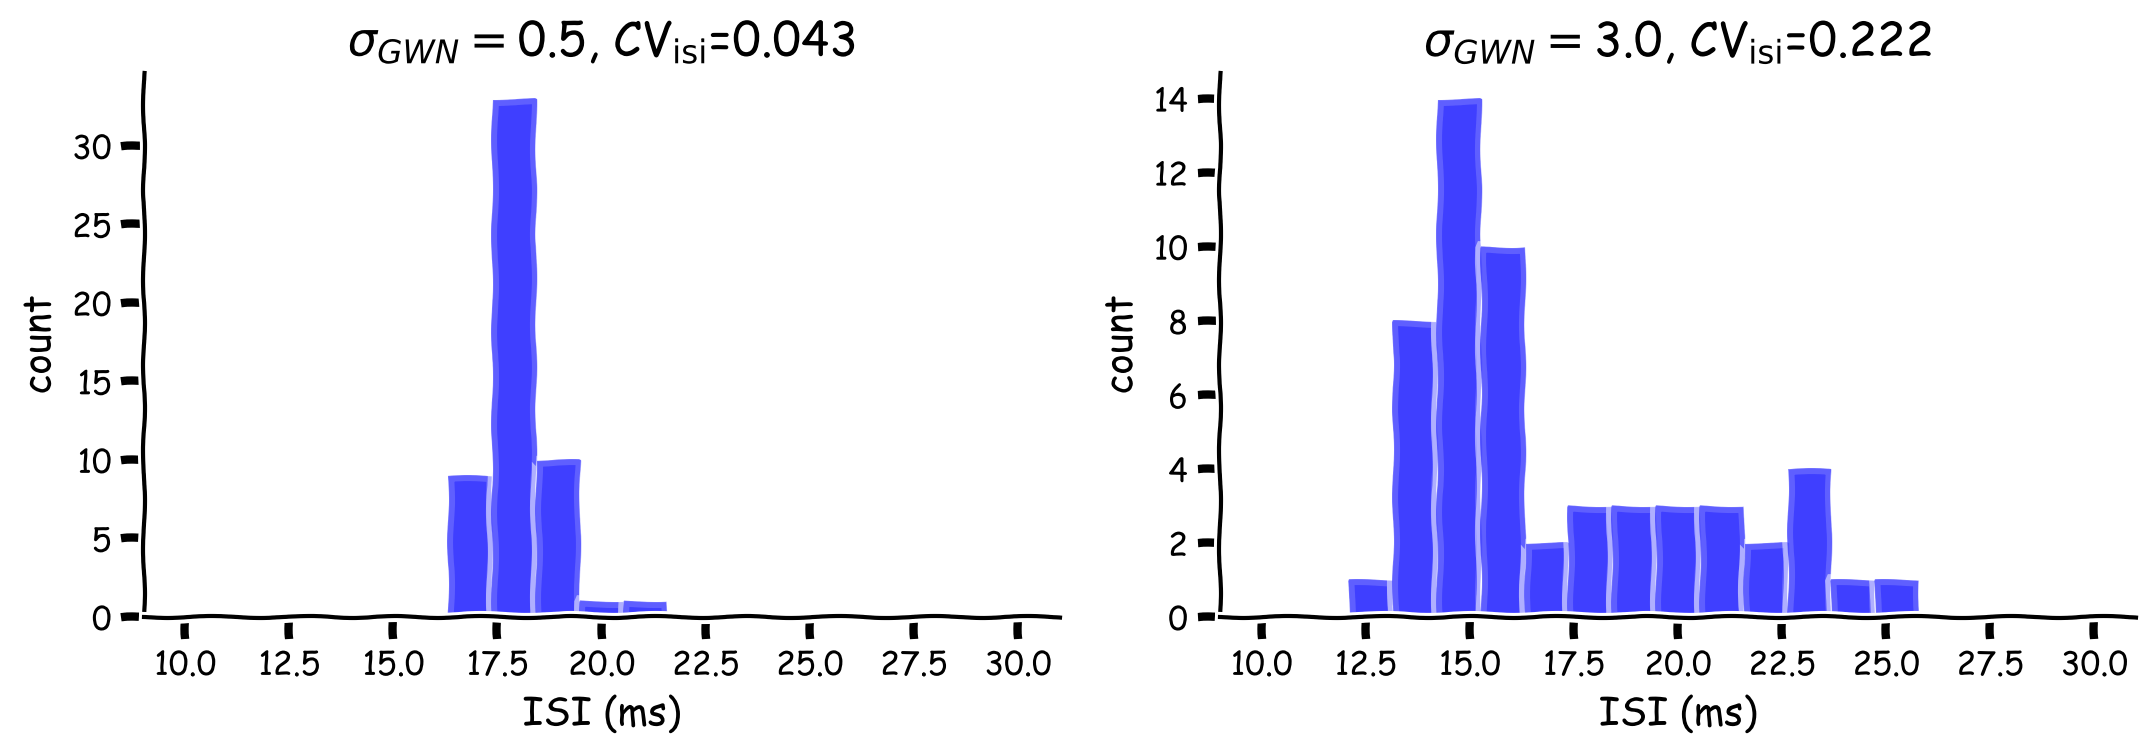
\includegraphics[scale=0.09]{Figures/BNM/LIF_Figure4.png}
\end{subbox}

\begin{subbox}{subbox}{Summary 
}
\scriptsize
You've a leaky integrate-and-fire (LIF) neuron model from scratch, and studied its dynamics in response to various types of inputs, having:
\begin{itemize}
    \item 
 simulated the LIF neuron model
\item 
 driven the LIF neuron with external inputs, such as direct current and Gaussian white noise

\item 
studied how different inputs affect the  LIF neuron's output (firing rate and spike time irregularity),
\end{itemize}

with a special focus on low rate and irregular firing regime to mimic real cortical neurons. The next tutorial will look at how spiking statistics may be influenced by a neuron's input statistics.

If you have extra time, look at the bonus sections below to explore a different type of noise input and learn about extensions to integrate-and-fire models.

\end{subbox}
\end{textbox}
%%%%%%%%%%%%%%%%%%%%%%%%%%%%%%%%%%%%%%%%%%%%%%%%%%%%%%
%%%%%%%%%%%%%%%%%%%%%%%%%%%%%%%%%%%%%%%%%%%%%%%%%%%%%%
% TUTORIAL 2
%%%%%%%%%%%%%%%%%%%%%%%%%%%%%%%%%%%%%%%%%%%%%%%%%%%%%%
%%%%%%%%%%%%%%%%%%%%%%%%%%%%%%%%%%%%%%%%%%%%%%%%%%%%%%
\begin{textbox}{\href{https://compneuro.neuromatch.io/tutorials/W1D4_GeneralizedLinearModels/student/W1D4_Tutorial1.html}{Effects of Input Correlation } }
\begin{subbox}{subbox}{Correlations (Synchrony)}
\scriptsize
Correlation or synchrony in neuronal activity can be described for any readout of brain activity. Here, we are concerned with the spiking activity of neurons. 

In the simplest way, correlation/synchrony refers to coincident spiking of neurons, i.e., when two neurons spike together, they are firing in \textbf{synchrony} or are \textbf{correlated}. Neurons can be synchronous in their instantaneous activity, i.e., they spike together with some probability. However, it is also possible that spiking of a neuron at time $t$ is correlated with the spikes of another neuron with a delay (time-delayed synchrony). 

\textbf{Origin of synchronous neuronal activity:}
\begin{itemize}
    \item 
 Common inputs, i.e., two neurons are receiving input from the same sources. The degree of correlation of the shared inputs is proportional to their output correlation.
 \item  Pooling from the same sources. Neurons do not share the same input neurons but are receiving inputs from neurons which themselves are correlated.
 \item  Neurons are connected to each other (uni- or bi-directionally): This will only give rise to time-delayed synchrony. Neurons could also be connected via gap-junctions.
 \item Neurons have similar parameters and initial conditions.
\end{itemize}

\textbf{Implications of synchrony}\\
When neurons spike together, they can have a stronger impact on downstream neurons. Synapses in the brain are sensitive to the temporal correlations (i.e., delay) between pre- and post-synaptic activity, and this, in turn, can lead to the formation of functional neuronal networks - the basis of unsupervised learning.

Synchrony implies a reduction in the dimensionality of the system. In addition, correlations, in many cases, can impair the decoding of neuronal activity.

A simple model to study the emergence of correlations is to inject common inputs to a pair of neurons and measure the output correlation as a function of the fraction of common inputs. 

Here, we are going to investigate the transfer of correlations by computing the correlation coefficient of spike trains recorded from two unconnected LIF neurons, which received correlated inputs.


The input current to LIF neuron $i$ $(i=1,2)$ is:

\begin{equation}
\frac{I_i}{g_L} =\mu_i + \sigma_i (\sqrt{1-c}\xi_i + \sqrt{c}\xi_c) \quad (1)
\end{equation}

where $\mu_i$ is the temporal average of the current. The Gaussian white noise $\xi_i$ is independent for each neuron, while $\xi_c$ is common to all neurons. The variable $c$ ($0\le c\le1$) controls the fraction of common and independent inputs. $\sigma_i$ shows the variance of the total input.

So, first, we will generate correlated inputs.

\end{subbox}

\end{textbox}
%%%%%%%%%%%%%%%%%%%%%%%%%%%%%%%%%%%%%%%%%%%%%%%%%%
%%%%%%%%%%%%%%%%%%%%%%%%%%%%%%%%%%%%%%%%%%%%%%%%%%
\begin{textbox}{\href{https://compneuro.neuromatch.io/tutorials/W1D4_GeneralizedLinearModels/student/W1D4_Tutorial1.html}{Effects of Input Correlation } }
\begin{subbox}{subbox}{Compute the correlation}
\scriptsize
The \textit{sample correlation coefficient} between two input currents $I_i$ and $I_j$ is defined as the sample covariance of $I_i$ and $I_j$ divided by the square root of the sample variance of $I_i$ multiplied with the square root of the sample variance of $I_j$. In equation form:  

\begin{align}
r_{ij} &= \frac{cov(I_i, I_j)}{\sqrt{var(I_i)} \sqrt{var(I_j)}}\\
cov(I_i, I_j) &= \sum_{k=1}^L (I_i^k -\bar{I}_i)(I_j^k -\bar{I}_j) \\
var(I_i) &= \sum_{k=1}^L (I_i^k -\bar{I}_i)^2
\end{align}

where $\bar{I}_i$ is the sample mean, k is the time bin, and L is the length of $I$.  This means that $I_i^k$ is current i at time $k\cdot dt$. Note that the equations above are not accurate for sample covariances and variances as they should be additionally divided by L-1 - we have dropped this term because it cancels out in the sample correlation coefficient formula.

The \textit{sample correlation coefficient} may also be referred to as the \textit{sample Pearson correlation coefficient}. Here, is a beautiful paper that explains multiple ways to calculate and understand correlations \href{https://www.stat.berkeley.edu/~rabbee/correlation.pdf}{Rodgers and Nicewander 1988.}

\centering
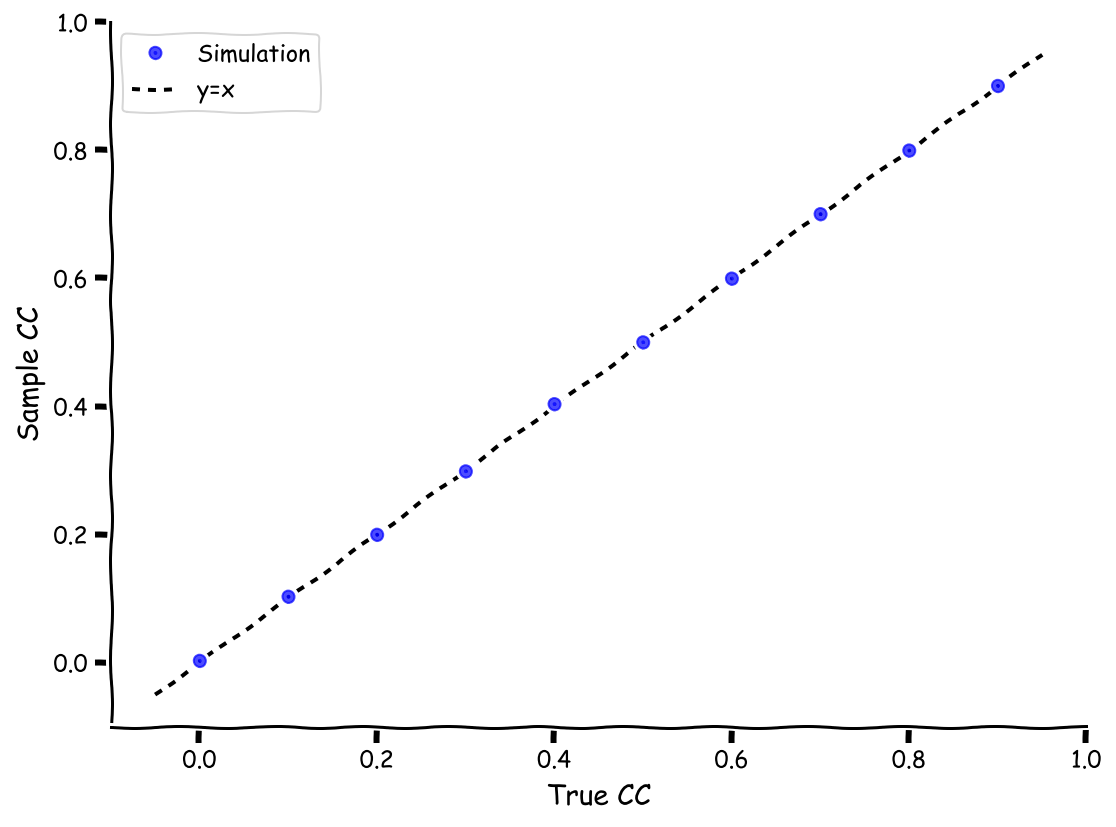
\includegraphics[scale=0.1]{Figures/BNM/LIF_Figure5.png}
\end{subbox}
\begin{subbox}{subbox}{Measure the correlation between spike trains}
\scriptsize

After recording the spike times of the two neurons, how can we estimate their correlation coefficient? 

In order to find this, we need to bin the spike times and obtain two time series. Each data point in the time series is the number of spikes in the corresponding time bin.

\begin{center}
    
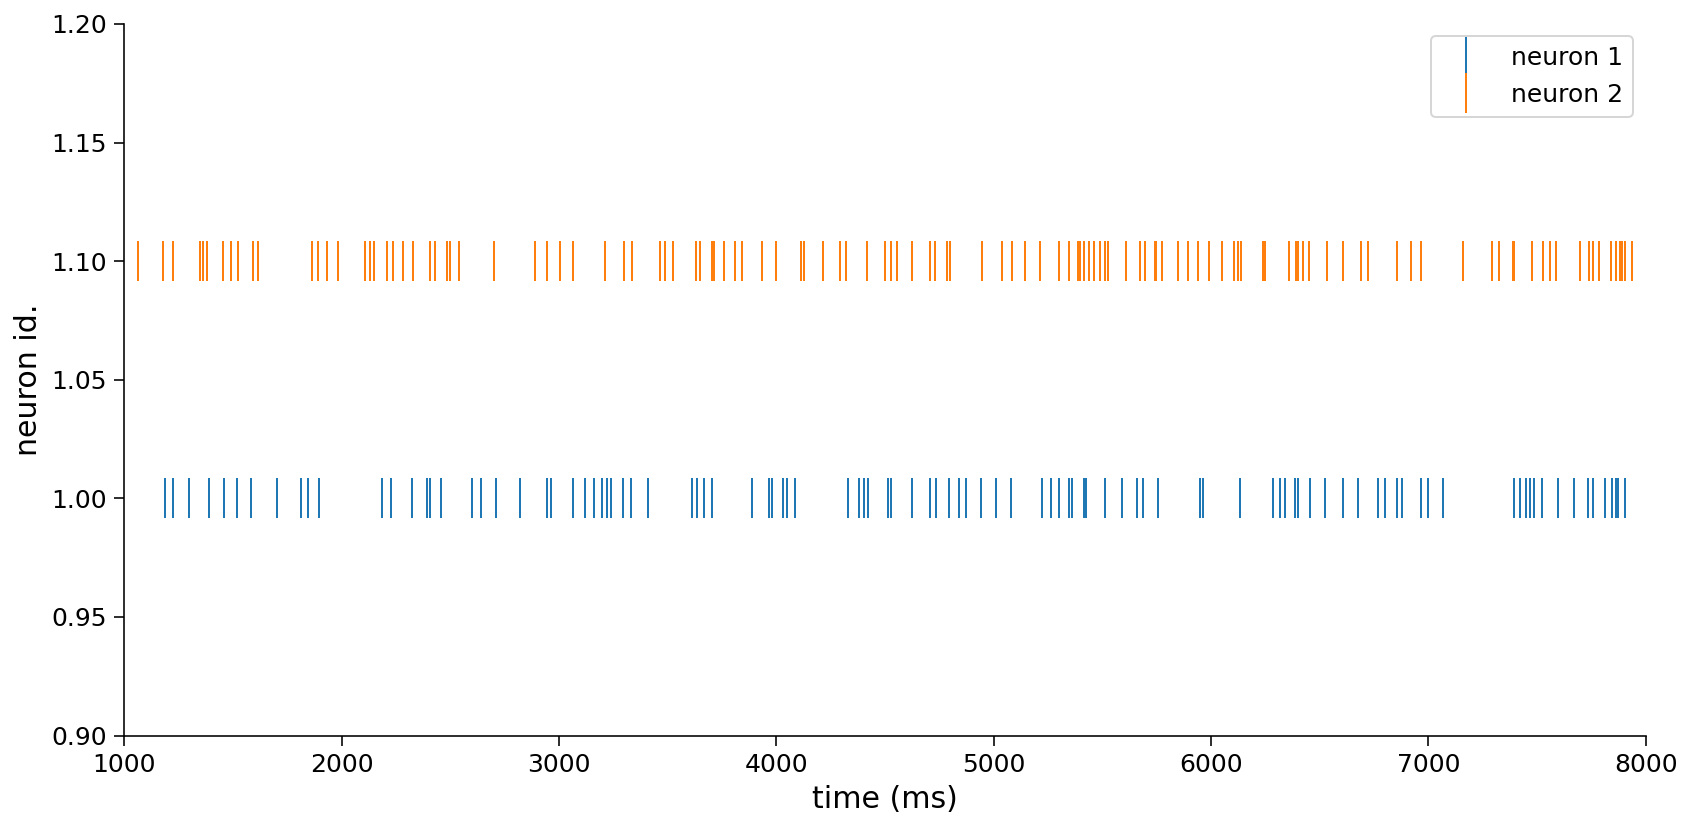
\includegraphics[scale=0.17]{Figures/BNM/LIF_Figure6.png}
\end{center}

\end{subbox}
\end{textbox}
%%%%%%%%%%%%%%%%%%%%%%%%%%%%%%%%%%%%%%%%%%%%%%%%%%
%%%%%%%%%%%%%%%%%%%%%%%%%%%%%%%%%%%%%%%%%%%%%%%%%%

\begin{textbox}{\href{https://compneuro.neuromatch.io/tutorials/W1D4_GeneralizedLinearModels/student/W1D4_Tutorial1.html}{Effects of Input Correlation } }


\begin{subbox}{subbox}{How do the mean and standard deviation of the Gaussian white noise (GWN) affect the correlation transfer function?}
\scriptsize
The correlations transfer function appears to be linear. The input/output transfer function of LIF neurons for correlations, instead of the transfer function for input/output firing rates.
What would you expect to happen to the slope of the correlation transfer function if you vary the mean and/or the standard deviation of the GWN of the inputs ?
\begin{center}
    
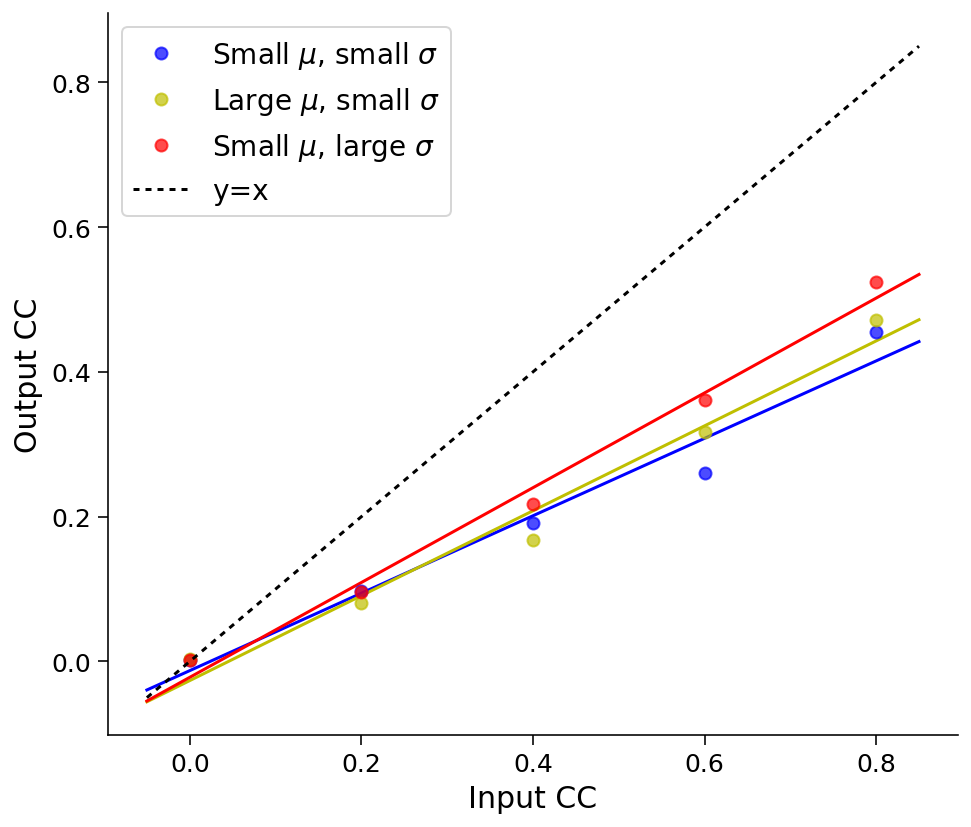
\includegraphics[scale=0.25]{Figures/BNM/LIF_Figure8.png}
\end{center}

\end{subbox}
\begin{subbox}{subbox}{
What is the rationale behind varying $\mu$ and $\sigma$?}
\scriptsize
The mean and the variance of the synaptic current depends on the spike rate of a Poisson process. We can use something called Campbell's theorem to estimate the mean and the variance of the synaptic current:
\begin{align}
\mu_{\rm syn} = \lambda J \int P(t) \\
\sigma_{\rm syn} = \lambda J \int P(t)^2 dt
\end{align}
%\begin{justify}
%\justifying
where $\lambda$ is the firing rate of the Poisson input, $J$ the amplitude of the postsynaptic current and $P(t)$ is the shape of the postsynaptic current as a function of time. 
Therefore, when we varied $\mu$ and/or $\sigma$ of the GWN, we mimicked a change in the input firing rate. Note that, if we change the firing rate, both $\mu$ and $\sigma$ will change simultaneously, not independently. 
Here, since we observe an effect of $\mu$ and $\sigma$ on correlation transfer, this implies that the input rate has an impact on the correlation transfer function.
%\end{justify}

%\end{flushleft}
\end{subbox}
\end{textbox}
%%%%%%%%%%%%%%%%%%%%%%%%%%%%%%%%%%%%%%%%%%%%%%%%%%
%%%%%%%%%%%%%%%%%%%%%%%%%%%%%%%%%%%%%%%%%%%%%%%%%%
% TUTORIAL 3
%%%%%%%%%%%%%%%%%%%%%%%%%%%%%%%%%%%%%%%%%%%%%%%%%%
%%%%%%%%%%%%%%%%%%%%%%%%%%%%%%%%%%%%%%%%%%%%%%%%%%

\begin{textbox}{\href{https://compneuro.neuromatch.io/tutorials/W2D3_BiologicalNeuronModels/student/W2D3_Tutorial3.html}{Synaptic transmission - Models of static and dynamic synapses } }


\begin{subbox}{subbox}{Static synapses}
\scriptsize
Synaptic input \textit{in vivo} consists of a mixture of \textbf{excitatory} neurotransmitters, which depolarizes the cell and drives it towards spike threshold, and \textbf{inhibitory} neurotransmitters that hyperpolarize it, driving it away from spike threshold. These chemicals cause specific ion channels on the postsynaptic neuron to open, resulting in a change in that neuron's conductance and, therefore, the flow of current in or out of the cell.

This process can be modeled by assuming that the presynaptic neuron's spiking activity produces transient changes in the postsynaptic neuron's conductance ($g_{\rm syn}(t)$). Typically, the conductance transient is modeled as an exponential function. 

Such conductance transients can be generated using a simple ordinary differential equation (ODE):

\begin{eqnarray}
\frac{dg_{\rm syn}(t)}{dt} &=& \bar{g}_{\rm syn} \sum_k \delta(t-t_k) -g_{\rm syn}(t)/\tau_{\rm syn}
\end{eqnarray}

where $\bar{g}_{\rm syn}$ (often referred to as synaptic weight) is the maximum conductance elicited by each incoming spike, and $\tau_{\rm syn}$ is the synaptic time constant. Note that the summation runs over all spikes received by the neuron at time $t_k$.

Ohm's law allows us to convert conductance changes to the current as:

\begin{align}
I_{\rm syn}(t) = g_{\rm syn}(t)(V(t)-E_{\rm syn}) 
\end{align}

The reversal potential $E_{\rm syn}$ determines the direction of current flow and the excitatory or inhibitory nature of the synapse. 

Thus, incoming spikes are filtered by an exponential-shaped kernel, effectively low-pass filtering the input. In other words, synaptic input is not white noise, but it is, in fact, colored noise, where the color (spectrum) of the noise is determined by the synaptic time constants of both excitatory and inhibitory synapses.

In a neuronal network, the total synaptic input current $I_{\rm syn}$ is the sum of both excitatory and inhibitory inputs. Assuming the total excitatory and inhibitory conductances received at time $t$ are $g_E(t)$ and $g_I(t)$, and their corresponding reversal potentials are $E_E$ and $E_I$, respectively, then the total synaptic current can be described as: 

\begin{align}
I_{\rm syn}(V(t),t) = -g_E(t) (V-E_E) - g_I(t) (V-E_I)
\end{align}


\end{subbox}
\end{textbox}
%%%%%%%%%%%%%%%%%%%%%%%%%%%%%%%%%%%%%%%%%%%%%
%%%%%%%%%%%%%%%%%%%%%%%%%%%%%%%%%%%%%%%%%%%%%

\begin{textbox}{\href{https://compneuro.neuromatch.io/tutorials/W2D3_BiologicalNeuronModels/student/W2D3_Tutorial3.html}{Synaptic transmission - Models of static and dynamic synapses } }
\begin{subbox}{subbox}{Static synapses}
\scriptsize

Accordingly, the membrane potential dynamics of the LIF neuron under synaptic current drive become:
\begin{eqnarray*}
\tau_m\frac{dV(t)}{dt} = -(V(t)-E_L) -\\ \frac{g_E(t)}{g_L} (V(t)-E_E) - \frac{g_I(t)}{g_L} (V(t)-E_I) + \frac{I_{\rm inj}}{g_L}\quad (\ddagger)
\end{eqnarray*}
$I_{\rm inj}$ is an external current injected in the neuron, which is under experimental control; it can be GWN, DC, or anything else.

We will use Eq. ($\ddagger$) to simulate the conductance-based LIF neuron model below.

In the previous tutorials, we saw how the output of a single neuron (spike count/rate and spike time irregularity) changes when we stimulate the neuron with DC and GWN, respectively. Now, we are in a position to study how the neuron behaves when it is bombarded with both excitatory and inhibitory spikes trains -- as happens \textit{in vivo}.

What kind of input is a neuron receiving? When we do not know, we choose the simplest option. The simplest model of input spikes is given when every input spike arrives independently of other spikes, i.e., we assume that the input is Poissonian.

\end{subbox}


\begin{subbox}{subbox}{Measure the mean free membrane potential}
\scriptsize
The conductance-based LIF neuron with presynaptic spike trains with rate 10 Hz for both excitatory and inhibitory inputs with 80 excitatory presynaptic spike trains and 20 inhibitory ones.

The $CV_{\rm ISI}$ can describe the irregularity of the output spike pattern. Now, we will introduce a new descriptor of the neuron membrane, i.e., the  \textbf{Free Membrane Potential (FMP)} -- the membrane potential of the neuron when its spike threshold is removed. 

Although this is completely artificial, calculating this quantity allows us to get an idea of how strong the input is. We are mostly interested in knowing the mean and standard deviation (std.) of the FMP. In the exercise, you can visualize the FMP and membrane voltage with spike threshold.
\begin{center}
    
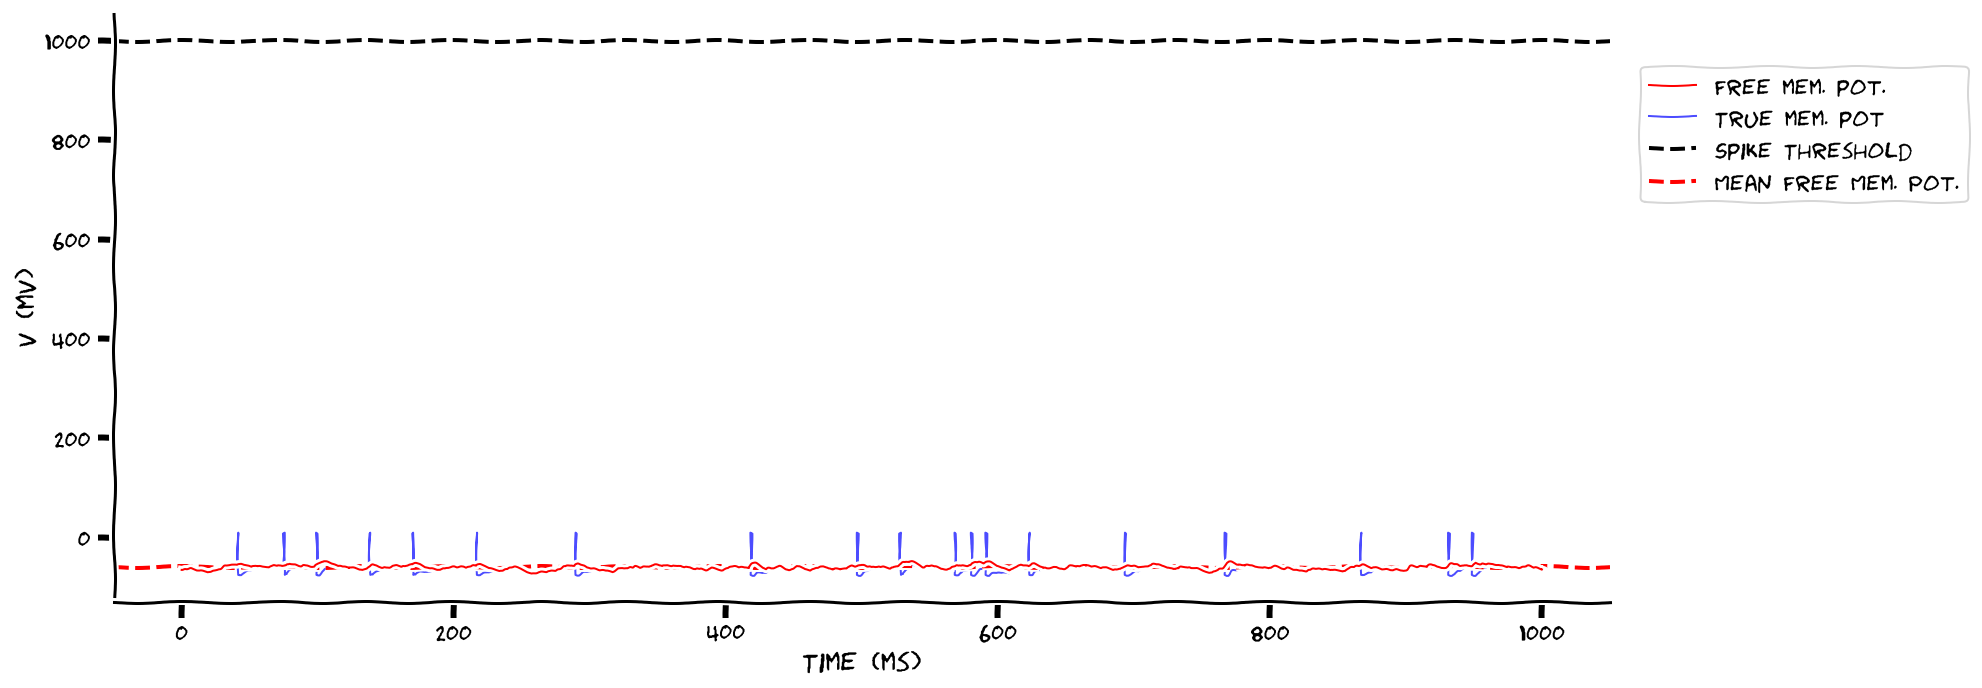
\includegraphics[scale=0.14]{Figures/BNM/LIF_Figure9.png}
\end{center}

\end{subbox}

\end{textbox}
%%%%%%%%%%%%%%%%%%%%%%%%%%%%%%%%%%%%%%%%%%%%%
%%%%%%%%%%%%%%%%%%%%%%%%%%%%%%%%%%%%%%%%%%%%%

\begin{textbox}{\href{https://compneuro.neuromatch.io/tutorials/W2D3_BiologicalNeuronModels/student/W2D3_Tutorial3.html}{Synaptic transmission - Models of static and dynamic synapses } }
\begin{subbox}{subbox}{Short-term synaptic plasticity}
\scriptsize
We modeled synapses with fixed weights. Now we will explore synapses whose weights change in some input conditions. 

Short-term plasticity (STP) is a phenomenon in which synaptic efficacy changes over time in a way that reflects the history of presynaptic activity. Two types of STP, with opposite effects on synaptic efficacy, have been experimentally observed. They are known as Short-Term Depression (STD) and Short-Term Facilitation (STF).

The mathematical model (for more information see \href{http://www.scholarpedia.org/article/Short-term_synaptic_plasticity}{here}) of STP is based on the concept of a limited pool of synaptic resources available for transmission ($R$), such as, for example, the overall amount of synaptic vesicles at the presynaptic terminals. The amount of presynaptic resource changes in a dynamic fashion depending on the recent history of spikes. 

Following a presynaptic spike, (i) the fraction $u$ (release probability) of the available pool to be utilized increases due to spike-induced calcium influx to the presynaptic terminal, after which (ii) $u$ is consumed to increase the post-synaptic conductance. Between spikes, $u$ decays back to zero with time constant $\tau_f$ and $R$ recovers to 1 with time constant $\tau_d$. In summary, the dynamics of excitatory (subscript $E$) STP are given by:
\begin{eqnarray*}
\frac{du_E}{dt} &=& -\frac{u_E}{\tau_f} + U_0(1-u_E^-)\delta(t-t_{\rm sp}) \\
\frac{dR_E}{dt} &=& \frac{1-R_E}{\tau_d} - u_E^+ R_E^- \delta(t-t_{\rm sp})  \\
\frac{dg_E(t)}{dt} &=& -\frac{g_E}{\tau_E} + \bar{g}_E u_E^+ R_E^- \delta(t-t_{\rm sp})
\end{eqnarray*}
where $U_0$ is a constant determining the increment of $u$ produced by a spike. $u_E^-$ and $R_E^-$ denote the corresponding values just before the spike arrives, whereas $u_E^+$ refers to the moment right after the spike. $\bar{g}_E$ denotes the maximum excitatory conductance, and $g_E(t)$ is calculated for all spike-times $k$, and decays over time with a time constant $\tau_{E}$. Similarly, one can obtain the dynamics of inhibitory STP (i.e., by replacing the subscript $E$ with $I$).
The interplay between the dynamics of $u$ and $R$ determines whether the joint effect of $uR$ is dominated by *depression* or *facilitation*. In the parameter regime of $\tau_d \gg \tau_f$  and for large $U_0$, an initial spike incurs a large drop in $R$ that takes a long time to recover; therefore, the synapse is STD-dominated. In the regime of $\tau_d \ll \tau_f$ and for small $U_0$, the synaptic efficacy is increased gradually by spikes, and consequently, the synapse is STF-dominated. This phenomenological model successfully reproduces the kinetic dynamics of depressed and facilitated synapses observed in many cortical areas.

\end{subbox}

\end{textbox}
%%%%%%%%%%%%%%%%%%%%%%%%%%%%%%%%%%%%%%%%%%%%%
%%%%%%%%%%%%%%%%%%%%%%%%%%%%%%%%%%%%%%%%%%%%%

\begin{textbox}{\href{https://compneuro.neuromatch.io/tutorials/W2D3_BiologicalNeuronModels/student/W2D3_Tutorial3.html}{Synaptic transmission - Models of static and dynamic synapses } }
\begin{subbox}{subbox}{Short-term synaptic depression (STD)}
\scriptsize
Below shows how Short-term synaptic depression (STD) changes for different firing rates of the presynaptic spike train and how the amplitude synaptic conductance $g$ changes with every incoming spike until it reaches its stationary state. 
\begin{center}
    
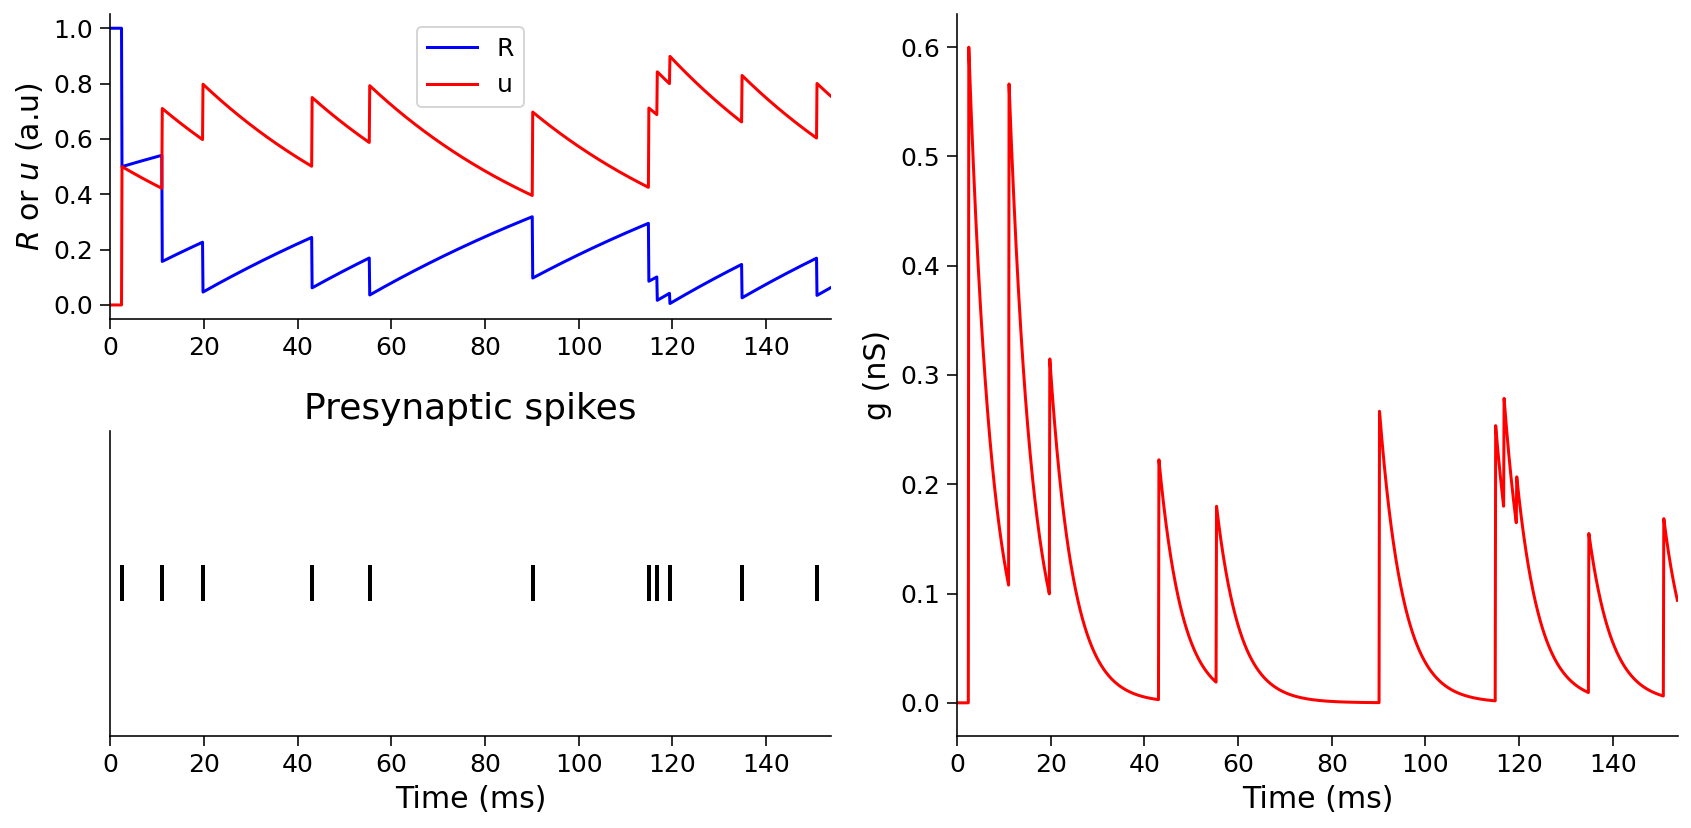
\includegraphics[scale=0.14]{Figures/BNM/LIF_Figure10.png}
\end{center}

Here, we will study how the ratio of the synaptic conductance corresponding to the first and 10th spikes change as a function of the presynaptic firing rate (experimentalists often take the ratio of first and second PSPs).

Below shows the STD conductance ratio with different input rates.
\begin{center}
    
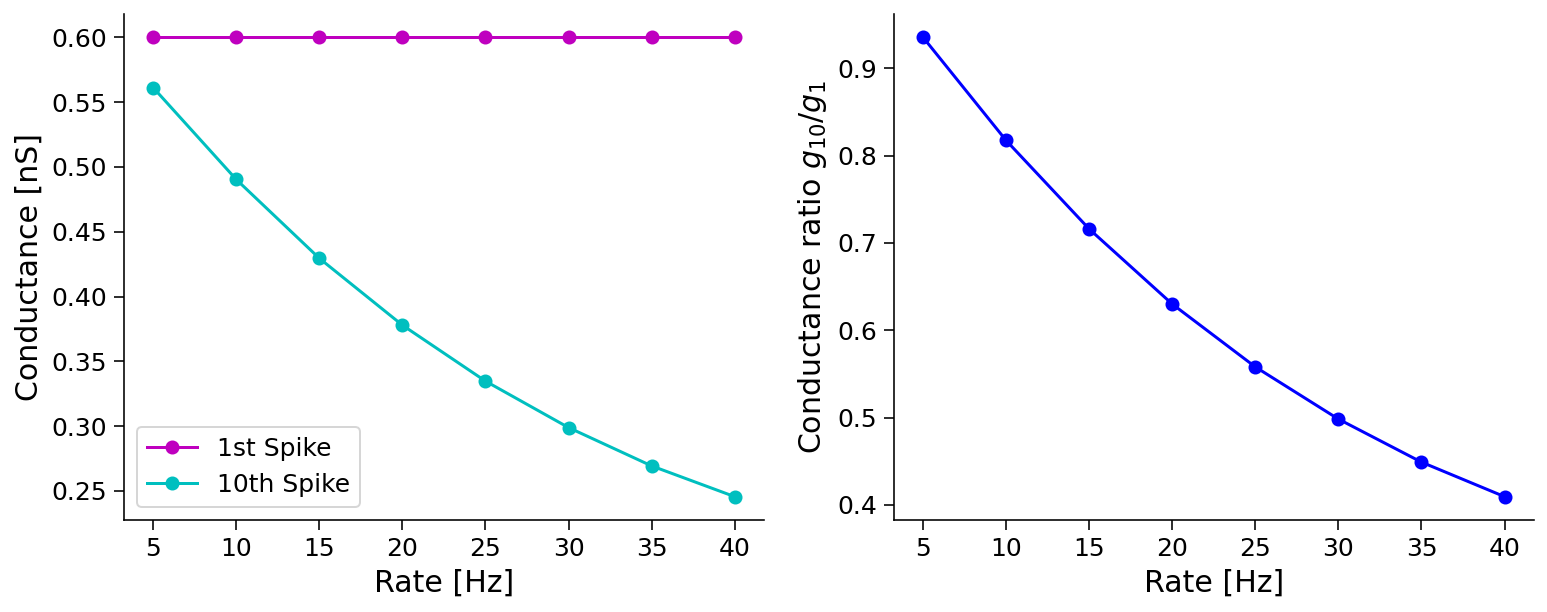
\includegraphics[scale=0.14]{Figures/BNM/LIF_Figure11.png}
\end{center}

\end{subbox}
\begin{subbox}{subbox}{Short-term synaptic facilitation (STF)}
\scriptsize
Below, we see an illustration of a short-term facilitation example. 

\begin{center}
    
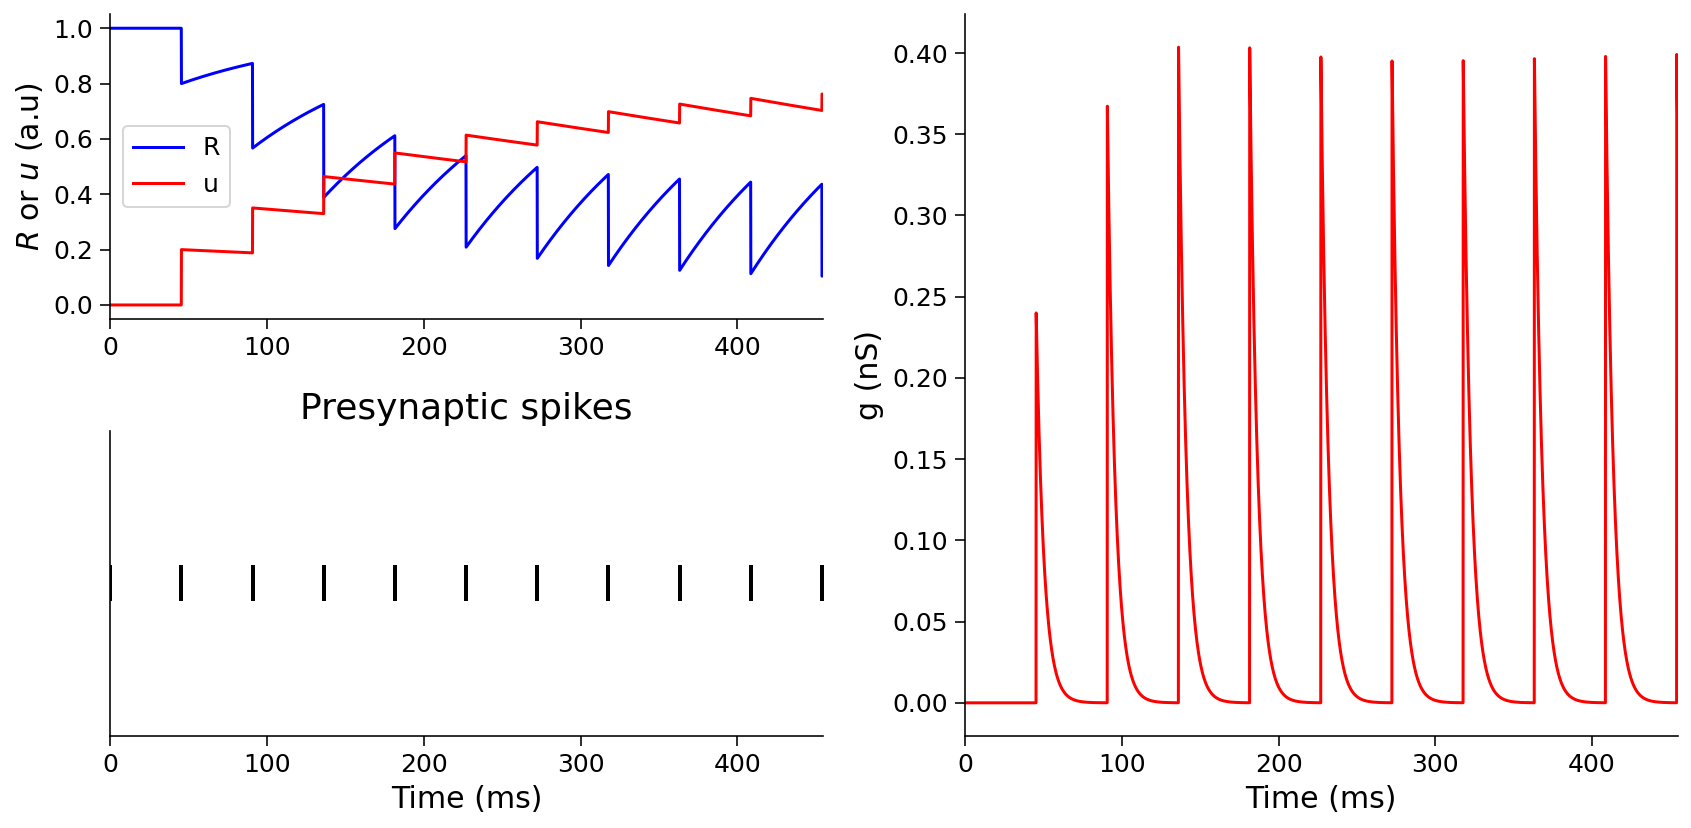
\includegraphics[scale=0.14]{Figures/BNM/LIF_Figure12.png}
\end{center}

Here, we will study how the ratio of the synaptic conductance corresponding to the $1^{st}$ and $10^{th}$ spike changes as a function of the presynaptic rate. 

Below STF conductance ratio with different input rates.
\begin{center}
    
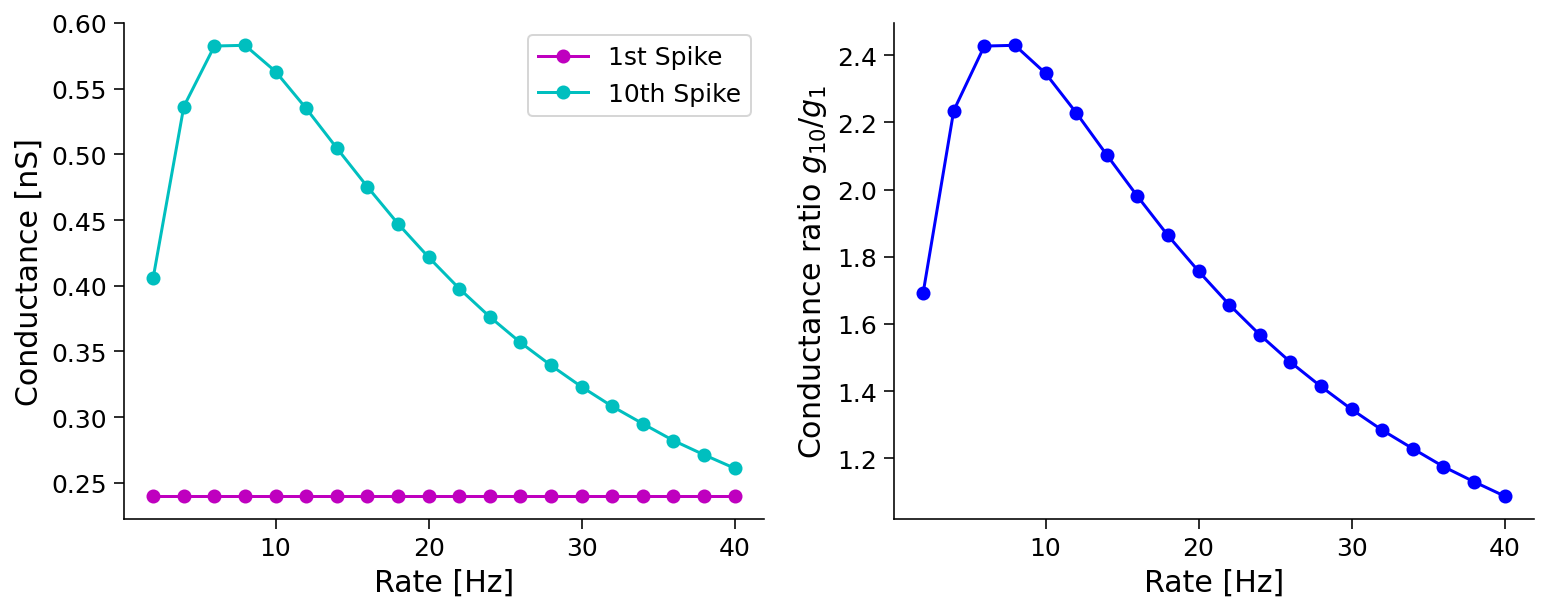
\includegraphics[scale=0.14]{Figures/BNM/LIF_Figure13.png}
\end{center}

\end{subbox}

\end{textbox}
